\documentclass[main.tex]{subfiles}
%% Current Author:
\usetikzlibrary{arrows.meta}
\setcounter{chapter}{11}
\begin{document}
\chapter{Electric Fields}
\begin{content}
  \item concept of an electric field
  \item uniform electric fields
  \item capacitance
  \item electric potential
  \item electric field of a point charge
\end{content}
\subsection{Candidates should be able to:}
\spec{explain what is meant by an electric field and recall and use $E=\frac{F}{q}$ for electric field strength}

An electric field is the region of space in which electrical forces are exerted on charged bodies. The definition of electric field strength is force per unit charge, and this is written in symbols as:
\[ E=\frac{F}{q} \]
Electric field therefore has units of \si{\newton\per\coulomb}.

\spec{recall that applying a potential difference to two parallel plates stores charge on the plates and produces a uniform electric field in the central region between them}

If an electric potential is created between two parallel plates a distance $d$ apart then an electric field exists between them. Except at the edges, the field is \emph{uniform}. This is shown in figure \ref{parallelplates} by the fact that the field lines are parallel.

\begin{figure}[ht]
  \begin{center}
    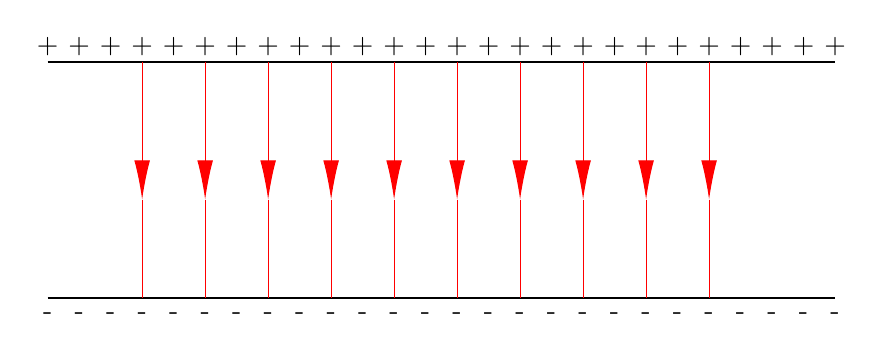
\begin{tikzpicture}
      \draw[thick] (0,0) -- (10,0);
      \draw[thick] (0,3) -- (10,3);
      \foreach \x in {1.2,2,...,8.8} {
        \draw[-{Latex[length=5mm, width=2mm]},red] (\x,3) -- (\x,1.25);
        \draw[red] (\x,1.25) -- (\x,0);
      }
      \foreach \x in {0,0.4,...,10} {
        \draw (\x,3.2) node {+};
        \draw (\x, -0.2) node {-};
      }
    \end{tikzpicture}
  \end{center}
  \caption{Uniform field between parallel plates}
  \label{parallelplates}
\end{figure}


Note that field lines show the direction in which a force would act on a \emph{postive} charge so they are from positive to negative.

\spec{derive and use the equations Fd = QV and $E=\frac{V}{d}$ for a charge moving through a potential difference in a uniform electric field}

From the definition potential difference we can say that the work done moving through a potential difference is \[ W = QV \] and that is equal to the force multiplied by the distance moved, \[ Fd \] If the movement is through a uniform field we can equate these two to give
\[ Fd = QV \]
The definition of electric field strength gives $F=QE$ and therefore substitution and re-arrangement give \[ E = \frac{V}{d} \]

\spec{recall that the charge stored on parallel plates is proportional to the potential difference between them}

This is an application of Gauss' law which relates the electric field strength around an object to the charge contained within a surface. It is enough to recall this fact at Pre-U.

\spec{recall and use $C = \frac{Q}{V}$ for capacitance}

This is the definition of capacitance and should be learnt. It can also be calculated from the gradient of a graph of $Q$ against $V$.

\spec{recognise and use $W = \frac{1}{2}QV$ for the energy stored by a capacitor, derive the equation from the area under a graph of charge stored against potential difference, and derive and use related equations such as $W = \frac{1}{2}CV^2$}

If a capacitor is partially charged with a charge $Q$ then to increase its potential difference by $\delta V$ will require a small amount of work $\delta W$ such that

\[ \delta W = Q \delta V  \]

If a graph is plotted of $Q$ against $V$ then this can be seen as the area of a small section. Thus, the energy required to charge a capacitor from uncharged to a p.d. of $V$ is given by the area of a graph of $Q$ against $V$ from zero to $V$, hence
\[ W = \frac{1}{2}QV \]

We can substitute for each quantity in turn to give the following variations of the equation:
\[ W = \frac{1}{2}QV = \frac{1}{2}CV^2 = \frac{1}{2}\frac{Q^2}{C} \]

This can, of course, also be done with integration
\[ W = \int_0^V Q dV = \int_0^V CV dV  = \frac{1}{2}CV^2 \]

\spec{analyse graphs of the variation with time of potential difference, charge and current for a capacitor discharging through a resistor}

When a capacitor discharges through a resistor the potential difference on the capacitor drives current around the circuit. Since it is this current which removes charge from the capacitor, it is the case that the rate of change of charge on the capacitor is proportional to the charge on the capacitor.

\[ \frac{dQ}{dt} = -I = -\frac{V}{R} = -\frac{Q}{RC} \]

This is a first order differential equation and has a solution

\[ Q = Q_0 e^{-\frac{t}{RC}} \]

The substitutions $Q=CV$ and then $I = \frac{V}{R}$ can be used to get similar equations for each of the above. The graph of this change is exponential decay. The key features are the initial value (e.g. $V_0$) and the fact that all three quantities tend to zero.

\spec{define and use the time constant of a discharging capacitor}

The time constant, $\tau$, is defines as follows:
\[ \tau = RC \]

This means that in one time constant the current, voltage and charge on a capacitor have declined to $\frac{1}{e}$ of their initial values.

A common rule-of-thumb from electronics is that a capacitor takes five time constants to discharge. If we plug this into the equation

\[ V = V_0 e^{-\frac{t}{RC}} = V_0 e^{-5} = 0.067\ V_0 \]

So the voltage across the capacitor has declined to less than 1\% of its initial value.

\spec{analyse the discharge of a capacitor using equations of the form $x=x_0e^{\frac{-t}{RC}}$}

Much of this has been covered above. One important point to note is that the analysis of capacitor decay is usually carried out by plotting a graph of $\ln{V}$ against time. This changes the equation to give
\[ \ln{V} = -\frac{t}{RC} + \ln{V_0} \]
Therefore the gradient of the graph is $-\frac{1}{RC}$ and the intercept $\ln{V_0}$.


\spec{understand that the direction and electric field strength of an electric field may be represented by field lines (lines of force), and recall the patterns of field lines that represent uniform and radial electric fields}

Field lines are a way of visualising the field. The direction of the field lines is from north to south and show the direction in which a positively charged particle will move. The density of field lines represent the strength of the field. For example in figure \ref{solenoid} the region \textbf{A} contains a uniform strong field which is stronger than the field at \textbf{B} as the field lines are more closely spaced.

\begin{figure}[ht]
	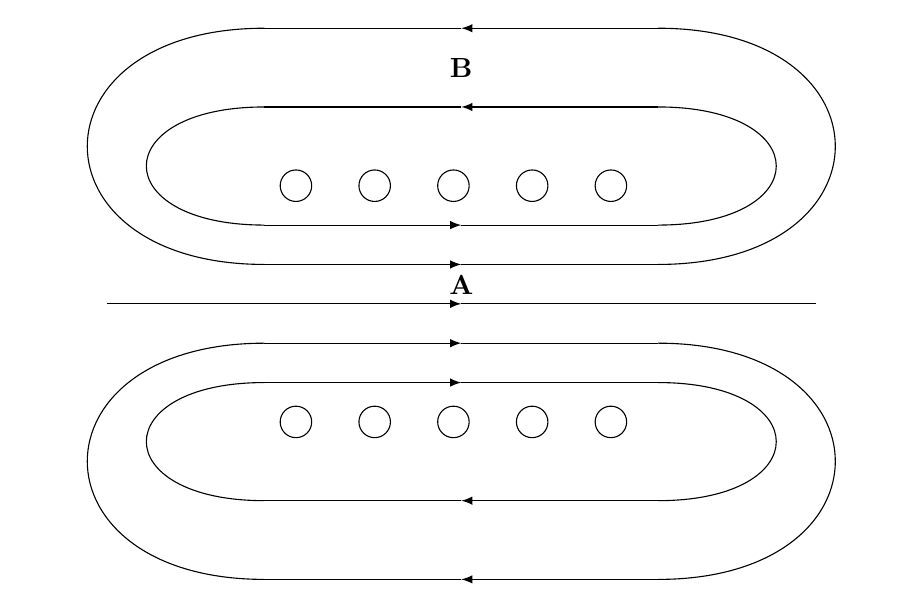
\begin{tikzpicture}
		\foreach \x in {1,2,3,4,5} {
			\draw (\x-0.6,0) circle (0.2cm);
			\draw (\x-0.6,3) circle (0.2cm);
		}
        % top loop
		\draw[-{latex[length=5mm,width=2mm]}] (0,2.5) -- (2.5,2.5);
		\draw (2.5,2.5) -- (5,2.5);
		\draw (5,2.5) .. controls (7,2.5) and (7,4) .. (5,4);
		\draw[-{latex[length=5mm,width=2mm]}] (5,4) -- (2.5,4);
		\draw (2.5,4) -- (0,4);
		\draw (0,4) .. controls (-2,4) and (-2,2.5) .. (0,2.5);
        % 2nd loop
		\draw[-{latex[length=5mm,width=2mm]}] (0,2) -- (2.5,2);
		\draw (2.5,2) -- (5,2);
		\draw (5,2) .. controls (8,2) and (8,5) .. (5,5);
		\draw[-{latex[length=5mm,width=2mm]}] (5,5) -- (2.5,5);
		\draw (2.5,5) -- (0,5);
		\draw (0,5) .. controls (-3,5) and (-3,2) .. (0,2);
        % middle loop
		\draw[-{latex[length=5mm,width=2mm]}] (-2,1.5) -- (2.5,1.5);
		\draw (2.5,1.5) -- (7,1.5);
        % 4th loop
		\draw[-{latex[length=5mm,width=2mm]}] (0,1) -- (2.5,1);
		\draw (2.5,1) -- (5,1);
		\draw (5,1) .. controls (8,1) and (8,-2) .. (5,-2);
		\draw[-{latex[length=5mm,width=2mm]}] (5,-2) -- (2.5,-2);
		\draw (2.5,-2) -- (0,-2);
		\draw (0,-2) .. controls (-3,-2) and (-3,1) .. (0,1);
        % bottom loop
		\draw[-{latex[length=5mm,width=2mm]}] (0,0.5) -- (2.5,0.5);
		\draw (2.5,0.5) -- (5,0.5);
		\draw (5,0.5) .. controls (7,0.5) and (7,-1) .. (5,-1);
		\draw[-{latex[length=5mm,width=2mm]}] (5,-1) -- (2.5,-1);
		\draw (2.5,-1) -- (0,-1);
		\draw (0,-1) .. controls (-2,-1) and (-2,0.5) .. (0,0.5);
        % Labels
        \draw (2.5,1.5) node[anchor=south] {\textbf{A}};
        \draw (2.5,4.5) node {\textbf{B}};
		
	\end{tikzpicture}
    \caption{Field around a solenoid}
    \ref{solenoid}
\end{figure}

\spec{understand electric potential and equipotentials}

Electric potential is defined as the energy per unit charge due to an electric field. Space without an electric field is defined as having zero potential. An equipotential is a line or surface on which the potential is a constant value. Therefore no work is done against the electric force moving along an equipotential. On diagrams equipotentials always cross field lines at right angles.

\spec{understand the relationship between electric field and potential gradient, and recall and use $E = -\frac{dV}{dX}$}

The strength of the electric field at any point is equal to the negative of the potential gradient. This can be seen most easily in a uniform field. If a unit charge is moved through a distance $\Delta x$ within a uniform field $E$ then the work down equals $Fx = -Ex$ (for a unit charge). The negative sign comes from the fact that if the force is doing work on the charge it must be moving in the opposite direction to the force on that charge. Thus, the change in energy per unit charge is given by $\Delta V = -E\Delta x$ or $E = -\frac{\Delta V}{Delta x}$. This can be generalised for a non-unform field as
\[ E = - \frac{dV}{dx} \]

\spec{recognise and use \[ F = \frac{Q_1 Q_2}{4\pi\epsilon_0 r^2} \] for point charges}

The equation above is known as Coulomb's law and enables the calculation of the force between two point charges separated by a distance $r$.

\spec{derive and use $E = \frac{Q}{4\pi\epsilon_o r^2} $ for the electric field due to a point charge}

This is simply from the definition of electric field strength:

\[ E = \frac{F}{Q} = \frac{1}{Q_2} \frac{Q_1 Q_2}{4\pi\epsilon_0 r^2} = \frac{Q}{4\pi\epsilon_o r^2} \]

\spec{*use integration to derive $W = \frac{Q_1 Q_2}{4\pi\epsilon_0 r}$ from $F=\frac{Q_1 Q_2}{4\pi\epsilon_0 r^2}$ for point charges}

Since free space is defined as having zero potential, the electrostatic potential energy, $W$, of a particle is equal to the work done by the field moving the particle from a distance $r$ to infinity. Since work done is equal to $\int F dx$ it follows:
\[ W = \int_{r}^\infty \frac{Q_1 Q_2}{4\pi\epsilon_0 r^2} dr = \frac{Q_1 Q_2}{4\pi\epsilon_0 r}\]

You can define this alternatively by thinking about the work done bringing a charged particle from infinity to a distance $r$. If you do this it is important to remember that $F$ acts in the opposite direction to $r$ so the limits of integration are reversed and the formula has a minus sign, thus reaching the same answer.

\spec{*recognise and use $W = \frac{Q_1 Q_2}{4\pi\epsilon_0 r }$ for the electrostatic potential energy for point charges.}

This is simply applying the equation above. This will allow the calculation of changes in potential energy and possibly transfer to other forms of energy (e.g. kinetic).

\end{document}
